\subsection{Night\-Set  Class Reference}
\label{class_nightset}\index{NightSet@{Night\-Set}}
a class representing a set of overlapping images of the same night, same instrument and same filter. 


{\tt \#include $<$reducedutils.h$>$}

Inheritance diagram for Night\-Set::\begin{figure}[H]
\begin{center}
\leavevmode
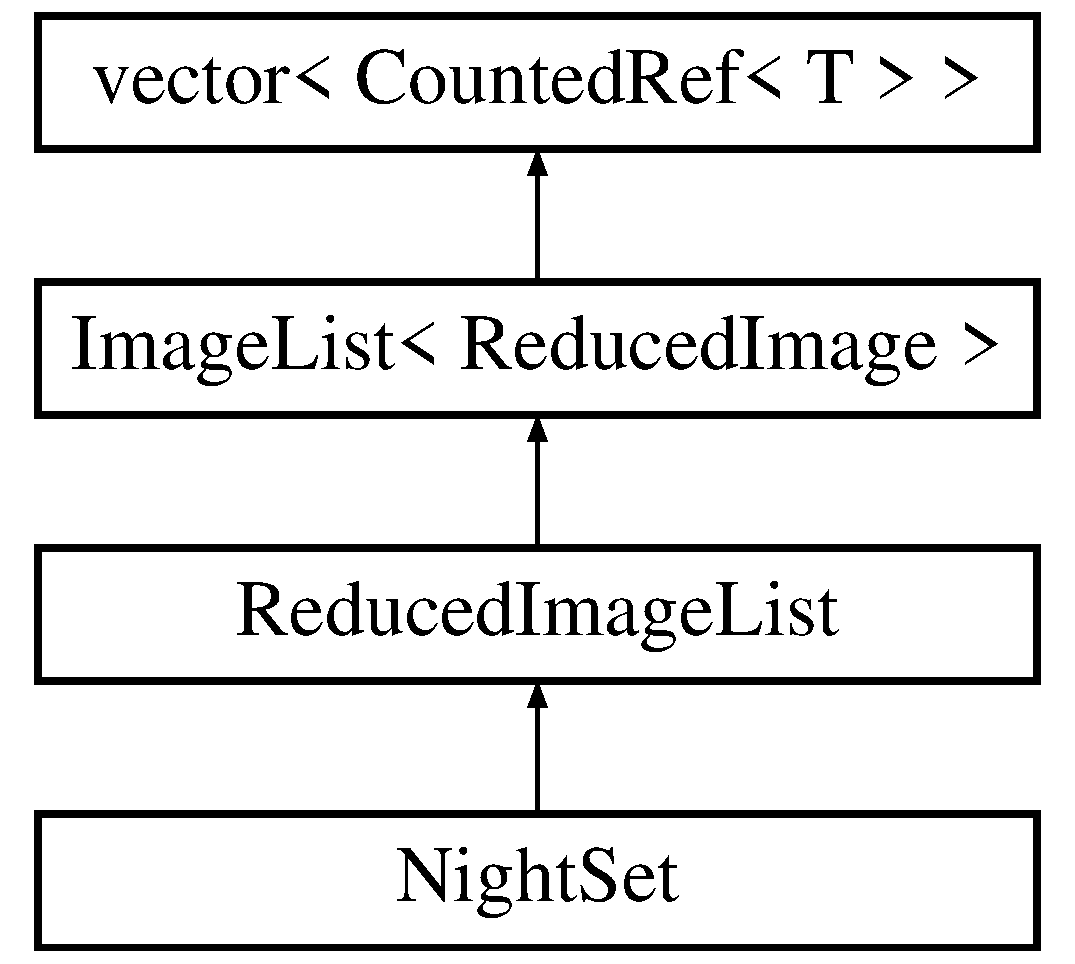
\includegraphics[height=4cm]{class_nightset}
\end{center}
\end{figure}
\subsubsection*{Public Methods}
\begin{CompactItemize}
\item 
\index{NightSet@{NightSet}!NightSet@{Night\-Set}}\index{NightSet@{NightSet}!NightSet@{Night\-Set}}
{\bf Night\-Set} (const {\bf Reduced\-Image} \&an\-Image)\label{class_nightset_a0}

\item 
\index{NightSet@{NightSet}!NightSet@{Night\-Set}}\index{NightSet@{NightSet}!NightSet@{Night\-Set}}
{\bf Night\-Set} (const Night\-Set \&Other)\label{class_nightset_a1}

\item 
\index{~NightSet@{$\sim$NightSet}!NightSet@{Night\-Set}}\index{NightSet@{NightSet}!~NightSet@{$\sim$Night\-Set}}
{\bf $\sim$Night\-Set} ()\label{class_nightset_a2}

\item 
\index{IsFromSameSet@{IsFromSameSet}!NightSet@{Night\-Set}}\index{NightSet@{NightSet}!IsFromSameSet@{Is\-From\-Same\-Set}}
bool {\bf Is\-From\-Same\-Set} (const {\bf Reduced\-Image} \&Another) const\label{class_nightset_a3}

\begin{CompactList}\small\item\em true if belongs to the same set.\item\end{CompactList}\item 
\index{GenericName@{GenericName}!NightSet@{Night\-Set}}\index{NightSet@{NightSet}!GenericName@{Generic\-Name}}
string {\bf Generic\-Name} () const\label{class_nightset_a4}

\begin{CompactList}\small\item\em returns the generic string name of the set.\item\end{CompactList}\item 
\index{dump@{dump}!NightSet@{Night\-Set}}\index{NightSet@{NightSet}!dump@{dump}}
void {\bf dump} (ostream \&Stream=cout) const\label{class_nightset_a5}

\item 
\index{Seeing@{Seeing}!NightSet@{Night\-Set}}\index{NightSet@{NightSet}!Seeing@{Seeing}}
double {\bf Seeing} () const\label{class_nightset_a6}

\item 
\index{Exposure@{Exposure}!NightSet@{Night\-Set}}\index{NightSet@{NightSet}!Exposure@{Exposure}}
double {\bf Exposure} () const\label{class_nightset_a7}

\item 
\index{SignalToNoise23@{SignalToNoise23}!NightSet@{Night\-Set}}\index{NightSet@{NightSet}!SignalToNoise23@{Signal\-To\-Noise23}}
double {\bf Signal\-To\-Noise23} () const\label{class_nightset_a8}

\end{CompactItemize}
\subsubsection*{Friends}
\begin{CompactItemize}
\item 
\index{operator<<@{operator$<$$<$}!NightSet@{Night\-Set}}\index{NightSet@{NightSet}!operator<<@{operator$<$$<$}}
ostream\& {\bf operator$<$$<$} (ostream \&Stream, const Night\-Set \&My\-Set)\label{class_nightset_l0}

\begin{CompactList}\small\item\em allows cout $<$$<$ Nigh\-Set;.\item\end{CompactList}\end{CompactItemize}


\subsubsection{Detailed Description}
a class representing a set of overlapping images of the same night, same instrument and same filter.



The documentation for this class was generated from the following file:\begin{CompactItemize}
\item 
{\bf reducedutils.h}\end{CompactItemize}
